% ---- pg-604 （书页 592） ----

\begin{mvtable}
\mvtabcap{表 5\quad $F$ 分布百分位点 $(\alpha=0.05)$}
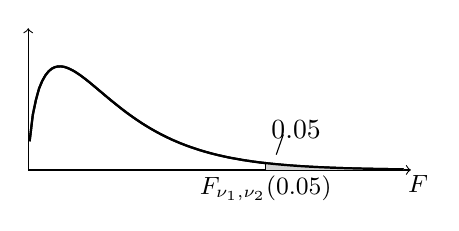
\begin{tikzpicture}[x=0.9cm,y=1.5cm]
% ---- 坐标轴 ----
\draw[->] (0,0) -- (5.4,0);
\draw[->] (0,0) -- (0,1.2);
% ---- F 分布密度曲线（近似） ----
\draw[thick,domain=0.02:5.3,samples=120]
  plot (\x,{2.6*(\x)^(0.6)*exp(-1.35*\x)});
% ---- 右侧阴影区 ----
\fill[gray!35]
  (3.35,0) -- plot[domain=3.35:5.3,samples=60]
  (\x,{2.6*(\x)^(0.6)*exp(-1.35*\x)}) -- (5.3,0) -- cycle;
\draw[thick,domain=0.02:5.3,samples=120]
  plot (\x,{2.6*(\x)^(0.6)*exp(-1.35*\x)});
% ---- 分位点竖线 ----
\draw (3.35,0) -- (3.35,{2.6*(3.35^0.6)*exp(-1.35*3.35)});
% ---- 标注 ----
\draw (3.6,0.30) -- (3.5,0.13);
\node[inner sep=1pt] at (3.78,0.34) {$0.05$};
% ---- 轴标签 ----
\node[below,inner sep=1pt,font=\small] at (3.35,-0.02) {$F_{\nu_{1},\nu_{2}}(0.05)$};
\node[below,inner sep=1pt,font=\small] at (5.5,-0.02) {$F$};
\end{tikzpicture}

{\zihao{6}
\mvfit{%
\begin{tabular}{r|*{17}{r}}
\toprule
\makecell{$\nu_{1}$\\$\nu_{2}$} & 1 & 2 & 3 & 4 & 5 & 6 & 7 & 8 & 9 & 10 & 12 & 15 & 20 & 25 & 30 & 40 & 60\\
\midrule
1 & 161.5 & 199.5 & 215.7 & 224.6 & 230.2 & 234.0 & 236.8 & 238.9 & 240.5 & 241.9 & 243.9 & 246.0 & 248.0 & 249.3 & 250.1 & 251.1 & 252.2\\
2 & 18.51 & 19.00 & 19.16 & 19.25 & 19.30 & 19.33 & 19.35 & 19.37 & 19.38 & 19.40 & 19.41 & 19.43 & 19.45 & 19.46 & 19.46 & 19.47 & 19.48\\
3 & 10.13 & 9.55 & 9.28 & 9.12 & 9.01 & 8.94 & 8.89 & 8.85 & 8.81 & 8.79 & 8.74 & 8.70 & 8.66 & 8.63 & 8.62 & 8.59 & 8.57\\
4 & 7.71 & 6.94 & 6.59 & 6.39 & 6.26 & 6.16 & 6.09 & 6.04 & 6.00 & 5.96 & 5.91 & 5.86 & 5.80 & 5.77 & 5.75 & 5.72 & 5.69\\
5 & 6.61 & 5.79 & 5.41 & 5.19 & 5.05 & 4.95 & 4.88 & 4.82 & 4.77 & 4.74 & 4.68 & 4.62 & 4.56 & 4.52 & 4.50 & 4.46 & 4.43\\
6 & 5.99 & 5.14 & 4.76 & 4.53 & 4.39 & 4.28 & 4.21 & 4.15 & 4.10 & 4.06 & 4.00 & 3.94 & 3.87 & 3.83 & 3.81 & 3.77 & 3.74\\
7 & 5.59 & 4.74 & 4.35 & 4.12 & 3.97 & 3.87 & 3.79 & 3.73 & 3.68 & 3.64 & 3.57 & 3.51 & 3.44 & 3.40 & 3.38 & 3.34 & 3.30\\
8 & 5.32 & 4.46 & 4.07 & 3.84 & 3.69 & 3.58 & 3.50 & 3.44 & 3.39 & 3.35 & 3.28 & 3.22 & 3.15 & 3.11 & 3.08 & 3.04 & 3.01\\
9 & 5.12 & 4.26 & 3.86 & 3.63 & 3.48 & 3.37 & 3.29 & 3.23 & 3.18 & 3.14 & 3.07 & 3.01 & 2.94 & 2.89 & 2.86 & 2.83 & 2.79\\
10 & 4.96 & 4.10 & 3.71 & 3.48 & 3.33 & 3.22 & 3.14 & 3.07 & 3.02 & 2.98 & 2.91 & 2.85 & 2.77 & 2.73 & 2.70 & 2.66 & 2.62\\
11 & 4.84 & 3.98 & 3.59 & 3.36 & 3.20 & 3.09 & 3.01 & 2.95 & 2.90 & 2.85 & 2.79 & 2.72 & 2.65 & 2.60 & 2.57 & 2.53 & 2.49\\
12 & 4.75 & 3.89 & 3.49 & 3.26 & 3.11 & 3.00 & 2.91 & 2.85 & 2.80 & 2.75 & 2.69 & 2.62 & 2.54 & 2.50 & 2.47 & 2.43 & 2.38\\
13 & 4.67 & 3.81 & 3.41 & 3.18 & 3.03 & 2.92 & 2.83 & 2.77 & 2.71 & 2.67 & 2.60 & 2.53 & 2.46 & 2.41 & 2.38 & 2.34 & 2.30\\
14 & 4.60 & 3.74 & 3.34 & 3.11 & 2.96 & 2.85 & 2.76 & 2.70 & 2.65 & 2.60 & 2.53 & 2.46 & 2.39 & 2.34 & 2.31 & 2.27 & 2.22\\
15 & 4.54 & 3.68 & 3.29 & 3.06 & 2.90 & 2.79 & 2.71 & 2.64 & 2.59 & 2.54 & 2.48 & 2.40 & 2.33 & 2.28 & 2.25 & 2.20 & 2.16\\
\bottomrule
\end{tabular}
}}
\end{mvtable}
